% 多元函数微分章第6节：隐函数与反函数（隐函数定理、特征值与特征向量的局部微分、局部反函数定理）。

\section{隐函数与反函数}
\label{sec:analysis-implicit-parameter-integral}

前面各节对给定的显式映射求微分。本节反过来从方程出发：给定一组方程，判断它能否在基点附近确定唯一的函数，并求这个函数的导数。
实际问题中，变量之间常由约束联系，而不是由显式公式给出。单位圆上的点满足$x^2+y^2=1$，物理系统的平衡状态满足力的平衡方程，训练得到的最优参数满足梯度为零。我们关心的是：一部分变量（参数）稍作改变时，其余变量（未知量）是否随之唯一地、光滑地改变，变化率又是多少。
方程组用向量值映射表示。方程个数与待解变量个数相同时，关于待解变量的方阵Jacobian是否可逆，决定了能否在局部解出这些变量。本节先建立隐函数定理，再用它研究特征值和特征向量随矩阵的变化，最后得到局部反函数定理。

\subsection{隐函数的存在与微分}
\label{sec:multivariable-implicit-function}

显式函数直接给出输出，例如$y=\sqrt x$。关系$F(x,y)=0$则没有直接说明给定$x$时$y$取什么值：满足方程的$y$可能有多个，也可能一个都没有。

设$(a,b)$满足$F(a,b)=0$。若存在$a$附近的区间$I$、$b$附近的区间$J$和函数$\varphi:I\to J$，使得对$I\times J$中的点，$F(x,y)=0$成立恰好当$y=\varphi(x)$，就称方程在$(a,b)$附近确定了一个\term{隐函数}（implicit function）$y=\varphi(x)$。换句话说，只看$(a,b)$附近的小矩形，方程的解集恰是一个函数的图像。
因此先要说明局部解分支存在且唯一，然后才能对这条分支求导。

同一个方程在一些点附近确定隐函数，在另一些点附近则不确定。
\begin{example}[单位圆附近的隐函数]
\label{ex:multivariable-implicit-circle}
考虑单位圆$x^2+y^2-1=0$。在$(0,1)$附近，解集是上半圆$y=\sqrt{1-x^2}$的一段；在$(0,-1)$附近则是下半圆$y=-\sqrt{1-x^2}$的一段，两处都确定了隐函数。
但在$(1,0)$附近，每个略小于$1$的$x$对应上下两个解，略大于$1$的$x$没有解；无论矩形多小，解集都不是关于$x$的函数图像。此处圆的切线是竖直的。
\end{example}

解集分成几支时，还要指定从哪一个解出发。
\begin{example}[方程$y^2=x$的两支解]
\label{ex:multivariable-implicit-parabola-branches}
方程$y^2-x=0$在$x>0$时有正、负两支解$y=\pm\sqrt x$。固定其中一个非零解，例如$(1,1)$，可以在它附近选出唯一的正支。
但在$(0,0)$处两支相交，负$x$侧又没有实数解，因此不存在定义在含$0$的开区间上的解函数。
\end{example}

两个例子中不能局部解出$y$的点，都满足$\partial F/\partial y=2y=0$：单位圆在$(1,0)$处如此，$y^2-x$在$(0,0)$处也如此。下面的定理~\ref{thm:analysis-implicit-function}要求的可逆性，恰好在这些点失效。所以局部选解既要指定起始解，也要核对关于待解变量的导数。换一个被解变量，非退化条件也随之改变：单位圆在$(1,0)$处虽不能把$y$解成$x$的函数，却有$\partial F/\partial x=2\neq0$，可以在附近把$x$解成$y$的函数$x=\sqrt{1-y^2}$。

图~\ref{fig:vol1-add-implicit-branches}显示“局部唯一”怎样排除另一支解。在$(1,1)$附近只保留正支即可；在原点处，两支相交且负$x$没有实数解，不能这样局部选出可微的解。
\begin{figure}[!htb]
  \centering
  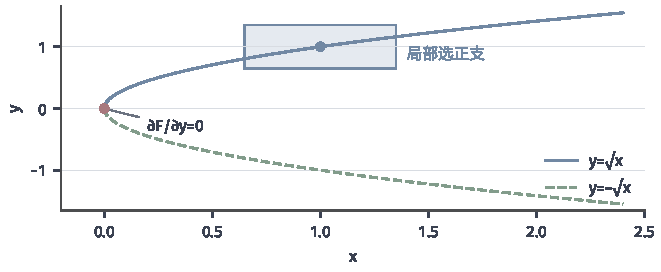
\includegraphics[width=112mm]{figures/00-shared/mathematical-preliminaries-upper/00-shared/matplotlib/mathematical-language-combinatorics-analysis-optimization-comprehension-additions/implicit-branches.pdf}
  \caption{方程$F(x,y)=y^2-x=0$的两支实数解。浅蓝矩形围住$(1,1)$，在该矩形内每个允许的$x$只有正支解，且$F_y=2y\neq0$；红点处$F_y=0$，两支相交。两支解满足同一方程，选定起始解与邻域才确定隐函数分支。}
  \label{fig:vol1-add-implicit-branches}
\end{figure}
\FloatBarrier


\paragraph{存在、唯一性与微分}

条件之所以落在关于待解变量的导数上，可以从线性方程看出来。

设$\bm x\in\mathbb R^p$为参数、$\bm y\in\mathbb R^m$为未知量，$\bm P\in\mathbb R^{m\times p}$、$\bm Q\in\mathbb R^{m\times m}$固定，方程$\bm P\bm x+\bm Q\bm y=\bm 0$有$m$个方程、$m$个未知量。当$\bm Q$可逆时，对每个$\bm x$都有唯一解$\bm y=-\bm Q^{-1}\bm P\bm x$；$\bm Q$不可逆时，对给定的$\bm x$，解要么不存在，要么不唯一。

对非线性方程$F(\bm x,\bm y)=\bm 0$，可微性说明它在基点附近近似于线性方程
\[
 \bm D_{\bm x}F(\bm a,\bm b)(\bm x-\bm a)+\bm D_{\bm y}F(\bm a,\bm b)(\bm y-\bm b)\approx\bm 0,
\]
其中$\bm D_{\bm x}F$、$\bm D_{\bm y}F$分别是只对$\bm x$、只对$\bm y$的坐标求偏导排成的Jacobian块。隐函数定理断言：只要线性近似中$\bm Q=\bm D_{\bm y}F$可逆，非线性方程在局部也像线性方程一样有唯一解，而且解的导数就是线性解的系数$-\bm Q^{-1}\bm P$。

定理给出的是充分条件。它只要求待解变量对应的方阵Jacobian可逆，不要求整个带参数映射的Jacobian是方阵。
\begin{theorem}[隐函数定理]
\label{thm:analysis-implicit-function}
设$F:\mathbb{R}^p\times\mathbb{R}^m\to\mathbb{R}^m$在$(\bm{a},\bm{b})$的某个开邻域内连续可微，$F(\bm{a},\bm{b})=\bm{0}$，并且关于待解变量的Jacobian矩阵
\[
 \bm{D}_{\bm{y}}F(\bm{a},\bm{b})\in\mathbb{R}^{m\times m}
\]
可逆。则存在$\bm{a}$与$\bm{b}$的邻域$U,V$，以及唯一的连续可微函数
$\varphi:U\to V$，使$\varphi(\bm{a})=\bm{b}$，并且对所有
$(\bm{x},\bm{y})\in U\times V$都有
\[
  F(\bm{x},\bm{y})=\bm{0}
  \quad\Longleftrightarrow\quad
  \bm{y}=\varphi(\bm{x}).
\]
其Jacobian矩阵满足
\begin{equation}
  \begin{aligned}
  \bm{D}\varphi(\bm{x})
  ={}&-\bigl[\bm{D}_{\bm{y}}F(\bm{x},\varphi(\bm{x}))\bigr]^{-1}\\
  &\cdot\bm{D}_{\bm{x}}F(\bm{x},\varphi(\bm{x})).
  \end{aligned}
\label{eq:analysis-implicit-derivative}
\end{equation}
\end{theorem}
矩阵形状为$(m\times m)(m\times p)=m\times p$，与$\varphi:\mathbb R^p\to\mathbb R^m$的Jacobian一致。唯一性只限于所选的邻域$U\times V$：定理不排除远处还有满足同一方程的其他解支，例如$y^2=x$在$(1,1)$附近选出正支，负支仍然存在。

若已知$\varphi$存在且可微，导数公式可以直接由链式法则得到：对恒等式$F(\bm x,\varphi(\bm x))=\bm 0$求导，得$\bm D_{\bm x}F+\bm D_{\bm y}F\,\bm D\varphi=\bm 0$，再左乘$(\bm D_{\bm y}F)^{-1}$。定理真正困难的部分是$\varphi$的存在、唯一与可微，形式求导不能替代这些步骤。

证明的思路是把解方程改写为反复修正的迭代。一元时，固定$x$，从$y_0=b$出发，用$y_{n+1}=y_n-F(x,y_n)/F_y(a,b)$不断修正：若$F(x,y_n)>0$且$F_y(a,b)>0$，就把$y$调小一点。这类似Newton法，只是斜率固定用基点处的值。若每次修正都使误差按固定比例缩小，迭代就收敛到唯一解。
证明依次检查三件事：修正映射是压缩；它不把点送出所考察的球；所得解随参数可微。
\begin{proof}
先把方程改写为局部压缩迭代。记
\[
 \begin{gathered}
\bm{A}=\bm{D}_{\bm{y}}F(\bm{a},\bm{b})\\
T_{\bm{x}}(\bm{y})=\bm{y}-\bm{A}^{-1}F(\bm{x},\bm{y}).
 \end{gathered}
\]
因为$\bm A^{-1}$可逆，$F(\bm{x},\bm{y})=\bm{0}$当且仅当$T_{\bm{x}}(\bm{y})=\bm{y}$，即$\bm y$是更新后保持不变的点，称为不动点。并且
\[
 \bm{D}_{\bm{y}}T_{\bm{x}}(\bm{y})=\bm{I}-\bm{A}^{-1}\bm{D}_{\bm{y}}F(\bm{x},\bm{y}),
\]
它在$(\bm{a},\bm{b})$处为零。由$F$的导数连续，这个矩阵的元素在基点附近都很小；又谱范数不超过Frobenius范数（第~\ref{sec:multivariable-operator-norm}节）。因而可以选择闭球$B=\{\bm{y}:\lVert\bm{y}-\bm{b}\rVert_2\leq r\}$和$\bm{a}$的邻域$U$，使
\begin{equation}
  \sup_{\bm{x}\in U,\,\bm{y}\in B}
  \left\lVert
    \bm{D}_{\bm{y}}T_{\bm{x}}(\bm{y})
  \right\rVert_2
  \leq q<1.
\label{eq:analysis-ift-uniform-contraction}
\end{equation}
沿$\bm{y}$方向使用式~\eqref{eq:analysis-operator-mean-value-bound}（球是凸集，球内线段不离开球）可知，每个
$T_{\bm{x}}$都把$B$内任意两点之间的距离缩小到原来的至多$q$倍。

还必须核对自映射，即$T_{\bm x}$不把$B$中的点送出$B$；否则迭代可能离开压缩成立的范围。因为$T_{\bm{a}}(\bm{b})=\bm{b}$且$T_{\bm{x}}(\bm{b})$关于$\bm{x}$连续，可进一步缩小$U$，使
\[
 \lVert T_{\bm{x}}(\bm{b})-\bm{b}\rVert_2\leq\frac{1-q}{2}r.
\]
于是对$\bm{y}\in B$，先用三角不等式拆开，再用压缩性，
\[
 \begin{aligned}
  \lVert T_{\bm{x}}(\bm{y})-\bm{b}\rVert_2
  &\leq
  \lVert T_{\bm{x}}(\bm{y})-T_{\bm{x}}(\bm{b})\rVert_2+\lVert T_{\bm{x}}(\bm{b})-\bm{b}\rVert_2\\
  &\leq
  q\lVert\bm{y}-\bm{b}\rVert_2+\frac{1-q}{2}r
  \leq
  \frac{1+q}{2}r
  <r.
 \end{aligned}
\]
所以$T_{\bm{x}}(B)$包含在$B$的内部$V$中。
固定$\bm x\in U$，从$\bm y_0=\bm b$出发，令$\bm y_{n+1}=T_{\bm x}(\bm y_n)$。
所有迭代项都留在$B$内，每一步的压缩使相邻差满足
$\lVert\bm y_{n+1}-\bm y_n\rVert_2\leq q\lVert\bm y_n-\bm y_{n-1}\rVert_2\leq\cdots\leq q^n\lVert\bm y_1-\bm y_0\rVert_2$。
增大$q$仍保留这个上界，因而可设$0<q<1$。对$m'>n$，几何和给出
\[
 \lVert\bm y_{m'}-\bm y_n\rVert_2
 \leq\sum_{j=n}^{m'-1}\lVert\bm y_{j+1}-\bm y_j\rVert_2
 \leq\frac{q^n}{1-q}\lVert\bm y_1-\bm y_0\rVert_2\longrightarrow0,
\]
所以$(\bm y_n)$是Cauchy列。有限维赋范空间完备（定理~\ref{thm:ls-finite-dimensional-complete}），该序列收敛；闭性使极限仍在$B$内。
$T_{\bm x}$连续，在$\bm y_{n+1}=T_{\bm x}(\bm y_n)$中令$n\to\infty$，可得极限$\varphi(\bm x)$满足
$T_{\bm x}(\varphi(\bm x))=\varphi(\bm x)$，而$T_{\bm x}(B)\subset V$使它属于$V$。
若另有不动点$\bm z\in B$，则
$\lVert\bm z-\varphi(\bm x)\rVert_2=\lVert T_{\bm x}(\bm z)-T_{\bm x}(\varphi(\bm x))\rVert_2\leq q\lVert\bm z-\varphi(\bm x)\rVert_2$，
由$q<1$只能有$\bm z=\varphi(\bm x)$，所以这个不动点唯一。若
$(\bm{x},\bm{y})\in U\times V$且$F(\bm{x},\bm{y})=\bm{0}$，则$\bm{y}\in B$也是
$T_{\bm{x}}$的不动点，唯一性迫使$\bm{y}=\varphi(\bm{x})$。这证明了定理所述的局部
存在与零点集合的逐点唯一性。

还需说明所得解随参数连续可微。先证$\varphi$局部Lipschitz连续，即它不会随参数剧烈变化。把$U$进一步缩小为开球，并使
$\overline U\times B$包含在原定义域内；这个集合闭且有界，$T_{\bm x}(\bm y)$关于$\bm x$的导数$-\bm A^{-1}\bm D_{\bm x}F$各分量连续，
故有统一范数上界$L$。对$\bm x,\bm x'\in U$，
两点间的线段仍在$U$内，式~\eqref{eq:analysis-operator-mean-value-bound}
可用于$T_{\bm x}(\bm y)$的参数变化。利用两个不动点关系$\varphi(\bm x)=T_{\bm x}(\varphi(\bm x))$、$\varphi(\bm x')=T_{\bm x'}(\varphi(\bm x'))$，把差拆成“改变$\bm y$”与“改变$\bm x$”两步：
\[
 \begin{aligned}
 \lVert\varphi(\bm{x})-\varphi(\bm{x}')\rVert_2
 &\leq\lVert T_{\bm x}(\varphi(\bm x))-T_{\bm x}(\varphi(\bm x'))\rVert_2\\
 &\quad+\lVert T_{\bm x}(\varphi(\bm x'))-T_{\bm x'}(\varphi(\bm x'))\rVert_2\\
 &\leq q\lVert\varphi(\bm{x})-\varphi(\bm{x}')\rVert_2+L\lVert\bm{x}-\bm{x}'\rVert_2,
 \end{aligned}
\]
移项得到$\lVert\varphi(\bm x)-\varphi(\bm x')\rVert_2
\leq L\lVert\bm x-\bm x'\rVert_2/(1-q)$，
故$\varphi$局部Lipschitz连续。

再证可微。令$\bm{h}\to\bm{0}$并记$\bm{k}=\varphi(\bm{x}+\bm{h})-\varphi(\bm{x})$，前述界给出$\lVert\bm{k}\rVert_2=O(\lVert\bm{h}\rVert_2)$。两点都在解集上，所以
\[
 F(\bm{x}+\bm{h},\varphi(\bm{x})+\bm{k})-F(\bm{x},\varphi(\bm{x}))=\bm{0}.
\]
对左侧作联合扰动$(\bm h,\bm k)$的一阶展开，得到
\[
 \bm{D}_{\bm{x}}F\,\bm{h}+\bm{D}_{\bm{y}}F\,\bm{k}+o(\lVert\bm{h}\rVert_2)=\bm{0}.
\]
展开中的Jacobian均在$(\bm x,\varphi(\bm x))$处取值，联合扰动的余项
$o(\lVert(\bm h,\bm k)\rVert_2)$因$\lVert\bm k\rVert_2=O(\lVert\bm h\rVert_2)$
成为$o(\lVert\bm h\rVert_2)$。
基点的$\det\bm A\neq0$，行列式又是矩阵元素的连续函数，
所以邻域足够小时$\bm D_{\bm y}F$仍可逆。左乘它的逆，得到
\[
 \bm{k}=-(\bm{D}_{\bm{y}}F)^{-1}\bm{D}_{\bm{x}}F\,\bm{h}+o(\lVert\bm{h}\rVert_2).
\]
这证明$\varphi$可微并给出式~\eqref{eq:analysis-implicit-derivative}；右侧各Jacobian矩阵及矩阵求逆都连续，又保证$\bm{D}\varphi$连续。至此，隐函数定理中的存在、局部唯一与导数公式都已得到证明。
\end{proof}

\paragraph{隐函数的导数}

定理成立后，计算隐函数的导数只需在选定分支上代入两个Jacobian。下面回到示例~\ref{ex:multivariable-implicit-parabola-branches}和示例~\ref{ex:multivariable-implicit-circle}的方程，核对不同分支各自的变化率。

\begin{example}[隐函数分支的导数]
\label{ex:multivariable-implicit-branch-derivative}
设$F(x,y)=y^2-x$，在$(1,1)$处有$F=0$、$F_y=2\neq0$。
隐函数定理保证$(1,1)$附近的解可以唯一写成$y=\varphi(x)$，且
\[
 \begin{gathered}
\varphi'(x)=-\frac{F_x(x,\varphi(x))}{F_y(x,\varphi(x))}
 =\frac1{2\varphi(x)}\\
\varphi'(1)=\frac12.
 \end{gathered}
\]
直接选正支$\varphi(x)=\sqrt x$，求导同样得到$1/(2\sqrt x)$。
若在$(1,-1)$附近选负支，导数则为$-1/2$。

对单位圆$x^2+y^2=1$上半圆的一点$(x_0,y_0)$（$y_0>0$），同一公式给出$\varphi'(x_0)=-x_0/y_0$，不必先解出$y=\sqrt{1-x^2}$。
\end{example}

起始解不同，所追踪的函数也不同，所以导数公式要在选定分支上取值。单位圆的导数$-x_0/y_0$在$y_0\to0$时趋于无穷，这与$(1,0)$处的竖直切线相符，也与示例~\ref{ex:multivariable-implicit-circle}的结论一致：$(1,0)$附近不能把$y$解成$x$的函数。曲线$y=\varphi(x)$的切向量是$(1,\varphi'(x_0))^\top=(1,-x_0/y_0)^\top$，它与梯度$\nabla F=(2x_0,2y_0)^\top$正交，回应了第~\ref{sec:multivariable-gradient-inner-product}节梯度与等值曲线的关系；梯度非零正是隐函数定理所需的非退化条件。若Jacobian奇异，定理不能直接使用：这既不能断言不存在可微分支，也不能默认分支仍唯一而光滑，须另行分析。

\paragraph{与线性解映射的一致性}
隐函数公式可以用第~\ref{sec:multivariable-inverse-differential}节已经求出的解映射核对。把$(\bm A,\bm b)$拉直后看作参数、$\bm x$看作未知量，令$F(\bm A,\bm b,\bm x)=\bm A\bm x-\bm b$。关于未知量的Jacobian是$\bm A$，可逆时满足定理条件；关于参数的微分作用于$(\bm E,\bm f)$，给出$\bm E\bm x-\bm f$。由式~\eqref{eq:analysis-implicit-derivative}，解分支的微分为
\[
 (\bm E,\bm f)\mapsto-\bm A^{-1}(\bm E\bm x-\bm f)=\bm A^{-1}(\bm f-\bm E\bm x),
\]
与式~\eqref{eq:multivariable-solution-map-differential}一致。这里只是核对：线性方程有显式的解公式，解误差的有限界与一阶响应都已在前面得到，不需要隐函数定理。特征方程$\bm S\bm v=\lambda\bm v$则不同，特征值与特征向量一般没有这样的显式公式，下面要先用隐函数定理证明局部分支存在且可微，再求它的响应。

\subsection{特征值与特征向量的局部微分}
\label{sec:multivariable-eigen-differential}

特征值和特征向量由方程$\bm S\bm v=\lambda\bm v$确定，并不是矩阵元素的显式函数。隐函数定理可以说明：矩阵稍作变化时，特征值和特征向量在什么条件下随之可微地变化，变化率又是多少。

设实对称矩阵$\bm S_0\in\mathbb R^{d\times d}$有一个简单特征值$\lambda_0$，对应单位特征向量$\bm v_0$。简单是指这个特征值的代数重数为$1$；对实对称矩阵，这等价于其特征空间是一维的。即使规定长度为$1$，$\bm v_0$和$-\bm v_0$仍代表同一方向。为了在局部选定一支，我们要求附近的向量$\bm v$满足$\bm v_0^\top\bm v>0$。这里选出的只是一个局部分支，单位长度本身并不保证全局唯一。

把对称矩阵$\bm S$作为参数，选取其上三角元素作为独立坐标，便可把对称矩阵空间视为有限维欧氏空间。把向量$\bm v$和标量$\lambda$作为未知量，特征方程与单位长度条件合起来写成
\[
 F(\bm S,\bm v,\lambda)=
 \begin{pmatrix}\bm S\bm v-\lambda\bm v\\ (\bm v^\top\bm v-1)/2\end{pmatrix}=\bm0.
\]
这是$d+1$个方程、$d+1$个未知量。在$(\bm S_0,\bm v_0,\lambda_0)$处，关于$(\bm v,\lambda)$的导数作用于$(\bm h,\eta)$，其矩阵为
\[
 \begin{pmatrix}\bm S_0-\lambda_0\bm I&-\bm v_0\\
 \bm v_0^\top&0\end{pmatrix}.
\]
要用隐函数定理，需验证这个方阵可逆，即它只把零向量映为零。设它把$(\bm h,\eta)$映为零。先用$\bm v_0^\top$左乘第一行，利用对称性及$\bm S_0\bm v_0=\lambda_0\bm v_0$得到$\eta=0$；第二行给出$\bm v_0^\top\bm h=0$。此时$\bm h$既属于$\lambda_0$的特征空间，又与$\bm v_0$正交。由于特征值简单，只能有$\bm h=\bm0$。因此这个方阵可逆，隐函数定理保证在$\bm S_0$附近存在可微的特征值和单位特征向量分支；上述内积为正的条件固定了局部符号。

有了可微分支，就可以求它对每个小的对称扰动方向的一阶响应。设对称扰动方向$\bm E$使特征值与特征向量分别产生一阶变化$\mathrm d\lambda(\bm E)$和$\mathrm d\bm v(\bm E)$。对特征方程与归一化条件求微分，并在基点取值，得到
\[
 \begin{gathered}
(\bm S_0-\lambda_0\bm I)\,\mathrm d\bm v(\bm E)
 =-\bigl(\bm E-\mathrm d\lambda(\bm E)\bm I\bigr)\bm v_0\\
\bm v_0^\top\mathrm d\bm v(\bm E)=0.
 \end{gathered}
\]
用$\bm v_0^\top$左乘第一式，左侧为零，于是
\[
 \mathrm d\lambda(\bm E)=\bm v_0^\top\bm E\bm v_0.
\]
把它代回后，第一式右侧与$\bm v_0$正交。由于$\lambda_0$简单，$\bm S_0-\lambda_0\bm I$限制在$\bm v_0$的正交补上可逆，因此第二式选出了唯一的$\mathrm d\bm v(\bm E)$。这里的微分作用于全部小的对称方向；可微分支的存在由上一段的隐函数定理保证，形式求导本身不能承担这一步。

\paragraph{谱展开与谱隙}
在$\bm S_0$的标准正交特征基中，向量响应可以显式写出。设$\bm S_0\bm v_j=\lambda_j\bm v_j$（$j=1,\ldots,d$），$\bm v_1,\ldots,\bm v_d$标准正交，并记$\bm v_0=\bm v_i$、$\lambda_0=\lambda_i$。$\mathrm d\bm v(\bm E)$与$\bm v_i$正交，可写成$\sum_{j\neq i}c_j\bm v_j$。代入第一式，左侧为$\sum_{j\neq i}c_j(\lambda_j-\lambda_i)\bm v_j$；与$\bm v_j$（$j\neq i$）作内积，右侧给出$-\bm v_j^\top\bm E\bm v_i$，所以
\[
 \mathrm d\bm v(\bm E)=\sum_{j\neq i}\frac{\bm v_j^\top\bm E\bm v_i}{\lambda_i-\lambda_j}\,\bm v_j .
\]
设$d\geq2$，令谱隙$\gamma=\min_{j\neq i}|\lambda_i-\lambda_j|$，它因特征值简单而为正。由$\lVert\bm v_i\rVert_2=1$与谱范数的定义，$|\mathrm d\lambda(\bm E)|=|\bm v_i^\top\bm E\bm v_i|\leq\lVert\bm E\rVert_2$；由标准正交展开的Parseval等式，
\[
 \lVert\mathrm d\bm v(\bm E)\rVert_2^2=\sum_{j\neq i}\frac{(\bm v_j^\top\bm E\bm v_i)^2}{(\lambda_i-\lambda_j)^2}
 \leq\frac1{\gamma^2}\sum_{j}(\bm v_j^\top\bm E\bm v_i)^2=\frac{\lVert\bm E\bm v_i\rVert_2^2}{\gamma^2}\leq\frac{\lVert\bm E\rVert_2^2}{\gamma^2},
\]
即$\lVert\mathrm d\bm v(\bm E)\rVert_2\leq\lVert\bm E\rVert_2/\gamma$。$d=1$时单位特征向量分支恒为$\bm v_0$，微分为零。

这两个界可以与第~\ref{sec:ls-spectral-sensitivity}节比较。Weyl界与谱隙界控制的是有限扰动下特征值和特征子空间的整体变化；这里给出的是带方向的一阶响应。特征值的响应$\bm v_i^\top\bm E\bm v_i$只看扰动在该特征方向上的读数；特征向量的响应以$\lambda_i-\lambda_j$为分母，说明谱隙小时，扰动可以把特征向量大幅地转向相邻的特征方向。

\paragraph{重特征值}
上面的结论依赖所选特征值简单。重特征值使关于未知量的导数不可逆，因此不能直接沿用这个构造；但这只说明这条论证失效，并不断言每一条特征值分支都不可微，也不意味着矩阵多项式或可逆点处的求逆映射失去光滑性。第~\ref{sec:multivariable-local-condition-number}节的$\operatorname{diag}(t,-t)$说明，在重特征值处，排序后的特征值可以有有限条件数而不可微，未排序的分支却仍然光滑。研究重特征值附近时，应改为考察相应的特征子空间，而不是强行指定其中某一个特征向量；谱簇子空间的稳定性已在第~\ref{sec:ls-subspace-sensitivity}节处理，这里不重复谱扰动界。

\subsection{局部反函数与坐标变换}

隐函数定理还能回答反求输入的问题：已知映射$G$的输出$\bm y$，能否唯一确定产生它的输入$\bm x$，并且$\bm x$随$\bm y$光滑变化。例如由直角坐标$(x,y)$反求极坐标$(r,\theta)$。
线性映射$\bm y=\bm M\bm x$可逆当且仅当方阵$\bm M$可逆。非线性映射在一点附近近似于它的Jacobian，所以可以期待：Jacobian可逆时，映射在局部可逆。
把$G(\bm x)-\bm y=\bm 0$看成以输出为参数、输入为待解变量的一组方程，就能使用隐函数定理。
所得定理只给出两个邻域之间的逆映射，不断言$G$在整个定义域上单射。
\begin{theorem}[局部反函数定理]
\label{thm:multivariable-inverse-function}
设$U\subseteq\mathbb R^d$开，$G:U\to\mathbb R^d$连续可微，$\bm a\in U$，且$\bm J_G(\bm a)$可逆。
则存在$\bm a$的开邻域$U_0$与$G(\bm a)$的开邻域$V_0$，使$G:U_0\to V_0$为双射，逆映射连续可微，并满足
\[
 \bm J_{G^{-1}}(G(\bm x))=[\bm J_G(\bm x)]^{-1}
 \qquad(\bm x\in U_0).
\]
\end{theorem}
\begin{proof}
以输出$\bm y$为参数、原输入$\bm x$为待解变量，令$H(\bm y,\bm x)=G(\bm x)-\bm y$。
在$(G(\bm a),\bm a)$处，关于$\bm x$的Jacobian就是可逆的$\bm J_G(\bm a)$。隐函数定理给出开邻域$V_0$、$W$以及$C^1$映射$\varphi:V_0\to W$，使
\[
 G(\bm x)=\bm y\quad\Longleftrightarrow\quad\bm x=\varphi(\bm y)
 \qquad(\bm y\in V_0,\ \bm x\in W).
\]
将$W$缩小并重新选取$V_0$，可使$W\subset U$且$\bm J_G$在$W$内均可逆。
令$U_0=W\cap G^{-1}(V_0)$，它因$G$连续而为包含$\bm a$的开集。
每个$\bm y\in V_0$都有$G(\varphi(\bm y))=\bm y$，故$\varphi(\bm y)\in U_0$；反之，每个$\bm x\in U_0$都由上述唯一性满足$\varphi(G(\bm x))=\bm x$。
因此$G:U_0\to V_0$为双射，逆就是$C^1$映射$\varphi$。
对$G(\varphi(\bm y))=\bm y$使用链式法则，得到$\bm J_G(\varphi(\bm y))\bm J_\varphi(\bm y)=\bm I$，左乘逆矩阵便得到所述公式。
\end{proof}
公式说明，逆映射的局部伸缩恰好抵消原映射的局部伸缩。下面用极坐标映射具体验证。
\begin{example}[极坐标的局部反函数]
\label{ex:multivariable-polar-local-inverse}
对$P(r,\theta)=(r\cos\theta,r\sin\theta)^\top$，示例~\ref{ex:multivariable-polar-jacobian}算得$\det\bm J_P=r$，所以在$r>0$的每一点附近，都可以从$(x,y)$唯一、光滑地反求$(r,\theta)$。在$(r,\theta)=(2,\pi/2)$，即平面上的点$(0,2)$处，
\[
\begin{gathered}
\bm J_P=\begin{bmatrix}0&-2\\1&0\end{bmatrix}\\
\bm J_{P^{-1}}(0,2)=\bm J_P^{-1}=\begin{bmatrix}0&1\\-1/2&0\end{bmatrix}.
\end{gathered}
\]
第一行说明$\mathrm dr=\mathrm dy$：在正上方的点，向上移动直接增大半径。第二行说明$\mathrm d\theta=-\mathrm dx/2$：向左移动使角度增大，且因为半径为$2$，角度变化只有水平位移的一半。
\end{example}

在$r=0$处，Jacobian行列式为零，所有$\theta$都映到原点，确实无法反求$\theta$；这正是定理条件不满足的地方。

\paragraph{局部可逆与整体单射}

局部反函数定理是局部结论。即使Jacobian处处可逆，映射在整个定义域上也未必单射。
\begin{example}[Jacobian处处可逆而不单射]
\label{ex:multivariable-local-not-global-inverse}
考虑映射
\[
\begin{gathered}
g(u,v)=(e^u\cos v,e^u\sin v)^\top\\
(u,v)\in\mathbb R^2.
\end{gathered}
\]
它的Jacobian矩阵为
\[
\begin{gathered}
\bm J_g(u,v)=\begin{bmatrix}e^u\cos v&-e^u\sin v\\ e^u\sin v&e^u\cos v\end{bmatrix}\\
\det\bm J_g=e^{2u}>0,
\end{gathered}
\]
处处可逆。但$(u,v)$与$(u,v+2\pi)$给出同一输出，$g$不是单射。
\end{example}

这个$g$就是半径取$e^u$的极坐标映射。它在每一点附近可以反求，但沿$v$方向每隔$2\pi$就重复覆盖一次输出。

另一方面，有连续的逆也不保证逆可微。一元函数$x\mapsto x^3$全局单射，其逆$y\mapsto y^{1/3}$在$0$处没有有限导数；这对应$x^3$在$0$处导数为零，定理条件不满足。所以Jacobian非奇异的条件不能由整体单射代替；使用局部反函数定理时，邻域、可微性和Jacobian的可逆性都要逐项检查。下一章用坐标变换计算区域积分时（第~\ref{sec:classical-change-variables}节），还须检查所用区域上的一一对应、光滑性和边界的处理，不能仅凭一点处Jacobian非零就对整个区域换元。

\FloatBarrier
